\chapter{结构体}\label{ch09}

\emph{Long ago, when shepherds wanted to see if two herds of sheep were isomorphic, they would look for an explicit isomorphism}

\begin{flushright}
    ——John C. Baez and James Dolan, “\href{https://arxiv.org/abs/math/9802029}{Categorification}”
\end{flushright}

Rust的结构体,有时也称为\emph{structure},类似于C和C++中的\texttt{struct}类型、Python中的\texttt{class}、JavaScript中的对象。一个结构体把多个不同类型的值组合成单个值,所以你可以将它们作为一个单元进行处理。对于一个结构体,你可以读取并且修改它的各个组成部分。一个结构体也可以有一些关联的方法来操作它的组成部分。

Rust有三种类型的结构体:\emph{命名字段(name-field)}、\emph{类元组(tuple-like)}、\emph{类单元(unit-like)},它们的区别在于如何引用它们的组成部分:一个命名字段结构体给每一个组件取了一个名字,而类元组结构体用它们出现的顺序来标识它们。类单元结构体没有任何组成部分,它并不常见,但可能比你想象中的更加有用。

在这一章中我们将详细解释每一种结构体,并展示它们在内存中的布局。我们家给你介绍如何给它们添加方法、如何定义可以处理很多不同类型组件的泛型结构体、以及如何让Rust为你的结构体生成通用的trait的实现。

\section{命名字段结构体}

一个命名字段结构体的定义类似于这样:
\begin{minted}{Rust}
    /// 一个8位灰度像素的矩形
    struct GrayscaleMap {
        pixels: Vec<u8>,
        size: (usize, usize)
    }
\end{minted}

这里声明了一个结构体类型\texttt{GrayscaleMap},它有两个字段分别命名为\texttt{pixels}和\texttt{size}。Rust的一个习惯是所有的类型包括结构体,名称中的每一个单词的首字母大写,例如\texttt{GrayscaleMap},这种习惯称为\emph{大驼峰命名法}(或\emph{帕斯卡命名法})。字段和方法名都是小写,用下划线分隔每个单词。这被称为\emph{蛇形命名法}。

你可以用\emph{结构体表达式}构造一个这种类型的值,例如:
\begin{minted}{Rust}
    let width = 1024;
    let height = 576;
    let image = GrayscaleMap {
        pixels: vec![0; width * height],
        size: (width, height)
    };
\end{minted}

结构体表达式以类型名称开始(\texttt{GrayscaleMap}),然后在花括号中列出每一个字段的名称和值。还有一种缩写可以用同名的局部变量来充当字段:
\begin{minted}{Rust}
    fn new_map(size: (usize, usize), pixels: Vec<u8>) -> GrayscaleMap {
        assert_eq!(pixels.len(), size.0 * size.1);
        GrayscaleMap { pixels, size }
    }
\end{minted}

结构体表达式\texttt{GrayscaleMap \{ pixels, size \}}是\texttt{GrayscaleMap \{ pixels: pixels, size: size \}}的缩写。你也可以在使用同名字段缩写的同时使用\texttt{key: value}语法为其它字段赋值。

访问一个结构体的字段需要使用熟悉的\texttt{.}运算符:
\begin{minted}{Rust}
    assert_eq!(image.size, (1024, 476));
    assert_eq!(image.pixels.len(), 1024 * 576);
\end{minted}

和其他item一样,结构体默认是私有的,只在它们声明的模块及其子模块中可见。你可以通过在定义前加\texttt{pub}来让结构体在模块之外也可见。它的每一个字段也是这样,默认也是私有的:
\begin{minted}{Rust}
    /// 一个8位灰度像素的矩形
    pub struct GrayscaleMap {
        pub pixels: Vec<u8>,
        pub size: (usize, usize)
    }
\end{minted}

即使结构体被声明为\texttt{pub},它的字段也可以是私有的:
\begin{minted}{Rust}
    /// 一个8位灰度像素的矩形
    pub struct GrayscaleMap {
        pixels: Vec<u8>,
        size: (usize, usize)
    }
\end{minted}

其他的模块可以使用这个结构体和它的所有共有的关联函数,但不能通过字段名访问私有的字段,也不能通过结构体表达式创建新的\texttt{GrayscaleMap}值。也就是说,创建一个结构体的值要求所有的结构体字段都可见。这也是为什么你不能通过结构体表达式创建新的\texttt{String}或者\texttt{Vec}。这些标准类型都是结构体,但它们的字段全都是私有的。要想创建一个这些类型的值,你必须使用共有的类型关联函数,例如\texttt{Vec::new()}。

在创建一个命名字段结构体值的时候,你可以使用另一个相同类型的结构体来提供你省略的字段的值。在一个结构体表达式中,如果命名字段最后跟着一个\texttt{.. EXPR},那么没有提到的字段将从\texttt{EXPR}中获取值,\texttt{EXPR}必须是另一个相同类型的值。假设我们有一个代表游戏中的怪物的结构体:
\begin{minted}{Rust}
    // 在这个游戏中,连扫帚都有怪物。你将会看到。
    struct Boom {
        name: String,
        height: u32,
        health: u32,
        position: (f32, f32, f32),
        intent: BroomIntent
    }

    /// 一个`Broom`的工作状态有两种可能。
    #[derive(Copy, Clone)]
    enum BroomIntent { FetchWater, DumpWater }
\end{minted}

对程序员来说最好的童话是\emph{魔法师的学徒}:一个魔法师学徒制造了一把能替他工作的扫帚,但工作完成之后却不知道该如何停止它。用斧头把扫帚劈成两半会产生两把扫帚,每个只有一半大小,但仍然像之前一样盲目地继续工作:
\begin{minted}{Rust}
    // 以值接受输入的扫帚,会获取所有权
    fn chop(b: Broom) -> (Broom, Broom) {
        // 用`b`初始化`broom1`的大部分,只修改`height`。因为
        // `String`不是`Copy`,因此`broom1`会获取`b`的name的所有权。
        let mut broom1 = Broom { height: b.height / 2, .. b };

        // 用`broom1`初始化`broom2`的大部分。因为`String`不是
        // `Copy`,所以我们必须显式克隆`name`
        let mut broom2 = Broom { name: broom1.name.clone(), .. broom1 };

        // 给两半分别起不同的名字。
        broom1.name.push_str(" I");
        broom2.name.push_str(" II");
        (broom1, broom2)
    }
\end{minted}

这个定义完成之后,我们可以创建一个扫帚,将它劈成两半,然后我们会得到:
\begin{minted}{Rust}
    let hokey = Broom {
        name: "Hokey".to_string(),
        height: 60,
        width: 100,
        health: 100,
        position: (100.0, 200.0, 0.0),
        intent: BroomIntent::FetchWater
    };

    let (hokey1, hokey2) = chop(hokey);
    assert_eq!(hokey1.name, "Hokey I");
    assert_eq!(hokey1.height, 30);
    assert_eq!(hokey1.health, 100);

    assert_eq!(hokey2.name, "Hokey II");
    assert_eq!(hokey2.height, 30);
    assert_eq!(hokey2.health, 100);
\end{minted}

新的\texttt{hokey1}和\texttt{hokey2}扫帚接收到了新的调整之后的名字,高度减半,其他的值都和原来一样。

\section{类元组结构体}

第二种结构体类型称为\emph{类元组结构体},因为它类似一个元组:
\begin{minted}{Rust}
    struct Bounds(usize, usize);
\end{minted}

你可以像构建元组一样构造一个这种类型的值,除了必须要包含结构体的名字:
\begin{minted}{Rust}
    let image_bounds = Bounds(1024, 768);
\end{minted}

类元组结构体持有的值被称为\emph{元素},就像元组持有的值一样。你可以像访问元组的元素一样访问它们:
\begin{minted}{Rust}
    assert_eq!(image_bounds.0 * image_bounds.1, 786432);
\end{minted}

每一个类元组结构体的元素都可以是公有的或者私有的:
\begin{minted}{Rust}
    pub struct Bounds(pub usize, pub usize);
\end{minted}

表达式\texttt{Bounds(1024, 768)}看起来像一个函数调用,实际上它就是:定义这个类型也会隐式地定义一个同名函数:
\begin{minted}{Rust}
    fn Bounds(elem0: usize, elem1: usize) -> Bounds { ... }
\end{minted}

在底层,命名字段结构体和类元组结构体非常相似。到底用哪一个取决于可读性、二义性和简洁性。如果你将频繁使用\texttt{.}运算符来获取值的组成部分,那么通过名称来标识字段会增强可读性,也更不容易写错。如果你通常用模式匹配来获取元素,那么类元组结构体可以漂亮地完成工作。

类元组结构体常用于\emph{新类型},这种结构体只有单个组件,可以用来获得更严格的类型检查。例如如果你在处理只有ASCII的文本,你可以定义一个这样的新类型:
\begin{minted}{Rust}
    struct Ascii(Vec<u8>);
\end{minted}

使用这种类型表示ASCII字符串比简单的传递\texttt{Vec<u8>}缓冲区好得多,还可以在注释中表明这个类型到底是什么含义。新类型可以帮助Rust捕获其他字节缓冲区被传给期望ASCII文本的函数的错误。我们将在\hyperref[ch22]{第22章}中给出一个使用新类型来实现高效的类型转换的例子。

\section{类单元结构体}

第三种结构体有一点迷惑:它声明了一个没有任何元素的结构体类型:
\begin{minted}{Rust}
    struct Onesuch;
\end{minted}

一个这种类型的值不占用任何内存,类似于单元类型\texttt{()}。Rust不需要考虑怎么在内存中存储类单元结构体,也不需要生成操作它们的代码,因为它可以仅从其类型中得知它可能需要了解的有关值的所有信息。但从逻辑上讲,一个空的结构体和其他的有值的类型没有什么区别——或者更精确地说,一个这样的类型就是一个单独的值:
\begin{minted}{Rust}
    let o = Onesuch;
\end{minted}

当在“\nameref{field}”一节中介绍\texttt{..}运算符时,你已经遇到过一个类单元结构体了。表达式\texttt{3..5}是结构体值\texttt{Range \{ start: 3, end: 5 \}}的缩写,而表达式\texttt{..},两端都省略的情况下,就是类单元结构体值\texttt{RangeFull}的缩写。

当和trait一起使用时,类单元结构体会变得很有用。我们将在\hyperref[ch11]{第11章}中介绍trait。

\section{结构体布局}

在内存中,命名字段结构体和类元组结构体是同样的东西:一些可能不同类型的值的集合,以一种特殊的方式分布在内存中。例如,我们之前在这一章中定义的这个结构体:
\begin{minted}{Rust}
    struct GrayscaleMap {
        pixels: Vec<u8>,
        size: (usize, usize)
    }
\end{minted}

一个\texttt{GrayscaleMap}按照如\hyperref[f9-1]{图9-1}的布局分布在内存中。

\begin{figure}[htbp]
    \centering
    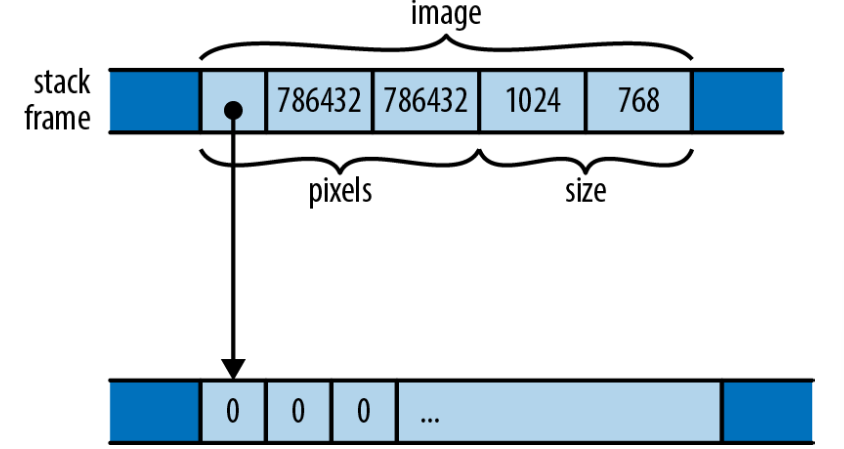
\includegraphics[width=0.8\textwidth]{../img/f9-1.png}
    \caption{一个\texttt{GrayscaleMap}结构体的内存布局}
    \label{f9-1}
\end{figure}

与C和C++不同,Rust对于如何在内存中布局结构体字段或元素没有任何确切的保证,这里的图只是展示了其中一种可能的排列。然而,Rust确实保证了直接在结构体的内存块里存储字段的值。JavaScript、Python和Java将会把\texttt{pixels}和\texttt{size}值分别放在它们自己的堆上分配的内存块中,然后让\texttt{GrayscaleMap}的字段指向他们。而Rust会直接把\texttt{pixels}和\texttt{size}嵌入到\texttt{GrayscaleMap}值里。只有\texttt{pixels} vector持有的堆上分配的缓冲区保留着自己的块。

你可以使用\texttt{\#[repr(C)]}属性来要求Rust用一种与C和C++兼容的方式布局结构体。我们将会在\hyperref[ch23]{第23章}中详细介绍这些。

\section{使用impl定义方法}\label{method}

整本书中,我们已经在很多类型的值上调用过方法。我们使用\texttt{v.push(e)}把元素添加进vector,使用\texttt{v.len()}获取它的长度,使用\texttt{r.expect("msg")}检查\texttt{Result}的值是否是错误值,等等。你可以为你自己的结构体类型定义方法。与C++或Java那种直接出现在结构体定义内部的方式不同,Rust的方法在一个单独的\texttt{impl}块中定义。

一个\texttt{impl}块就是一些\texttt{fn}定义的结合,每一个函数都将成为这个结构体的一个方法。例如,这里,我们定义了一个共有的结构体\texttt{Queue},然后为它定义了两个公有的方法:\texttt{push}和\texttt{pop}:
\begin{minted}{Rust}
    /// 一个先进先出的字符队列
    pub struct Queue {
        older: Vec<char>,   // 旧的元素,越旧越靠后
        younger: Vec<char>  // 新的元素,越新越靠后
    }

    impl Queue {
        /// 将一个字符添加到队列的尾部。
        pub fn push(&mut self, c: char) {
            self.younger.push(c);
        }

        /// 移出队列最前端的元素,如果有字符被移出就返回`Some(c)`,
        /// 否则如果队列为空就返回`None`。
        pub fn pop(&mut self) -> Option<char> {
            if self.older.is_empty() {
                if self.younger.is_empty() {
                    return None;
                }

                // 将新的元素都移动到旧的元素里,
                // 并且反转顺序。
                use std::mem::swap;
                swap(&mut self.older, &mut self.younger);
                self.older.reverse();
            }

            // 现在旧的元素保证不为空。Vec的pop方法
            // 已经返回了一个Option,因此不用再处理
            self.older.pop()
        }
    }
\end{minted}

在\emph{impl}块中定义的函数被称为\emph{关联函数},因为它们被关联到特定的类型。与之相反的是\emph{自由函数},也就是不在\texttt{impl}块中定义的函数。

Rust将调用方法的值作为第一个参数传给方法,它的参数名必须是\texttt{self}。因为\texttt{self}的类型很明显是\texttt{impl}块外面的结构体类型,或者是其引用,所以Rust允许你省略类型,用\texttt{self}、\texttt{\&self}、\texttt{\&mut self}分别作为\texttt{self: Queue}、\texttt{self: \&Queue}、\texttt{self: \&mut Queue}的缩写。如果你喜欢的话也可以使用非缩写的形式,但几乎所有的Rust都是用缩写形式。

在我们的示例中,\texttt{push}和\texttt{pop}方法中通过\texttt{self.older}和\texttt{self.younger}引用了\texttt{Queue}的字段。与C++或Java中“this”对象的成员直接在方法内可见不同,Rust方法中必须显式使用\texttt{self}来引用字段,这和Python方法中\texttt{self}的用法、JavaScript方法中\texttt{this}的用法类似。

因为\texttt{push}和\texttt{pop}需要修改\texttt{Queue},所以它们都以\texttt{\&mut self}传参。然而,当你调用这两个方法时,你不需要手动借用可变引用,普通的方法调用语法会自动进行隐式转换。因此有了这些定义之后,你可以像这样使用\texttt{Queue}:
\begin{minted}{Rust}
    let mut q = Queue { older: Vec::new(), younger: Vec::new() };

    q.push('0');
    q.push('1');
    assert_eq!(q.pop(), Some('0'));

    q.push('=');
    assert_eq!(q.pop(), Some('1'));
    assert_eq!(q.pop(), Some('='));
    assert_eq!(q.pop(), None);
\end{minted}

为了满足\texttt{push}方法的\texttt{self}参数要求,直接写\texttt{q.push(...)}会借用\texttt{q}的可变引用,就像你写了\texttt{(\&mut q).push(...)}一样。

如果一个方法不需要修改\texttt{self},那么你可以以共享引用获取参数。例如:
\begin{minted}{Rust}
    impl Queue {
        pub fn is_empty(&self) -> bool {
            self.older.is_empty() && self.younger.is_empty()
        }
    }
\end{minted}

方法调用表达式知道要借用哪一种引用:
\begin{minted}{Rust}
    assert!(q.is_empty());
    q.push('☉');
    assert!(!q.is_empty());
\end{minted}

或者,如果一个方法想获取\texttt{self}的所有权,它可以以值传递\texttt{self}:
\begin{minted}{Rust}
    impl Queue {
        pub fn split(self) -> (Vec<char>, Vec<char>) {
            (self.older, self.younger)
        }
    }
\end{minted}

调用这个\texttt{split}方法看起来和调用其他方法一样:
\begin{minted}{Rust}
    let mut q = Queue { older: Vec::new(), younger: Vec::new() };

    q.push('P');
    q.push('D');
    assert_eq!(q.pop(), Some('P'));
    q.push('X');

    let (older, younger) = q.split();
    // q现在是未初始化状态
    assert_eq!(older, vec!['D']);
    assert_eq!(younger, vec!['X']);
\end{minted}

但是注意,因为\texttt{split}以值获取\texttt{self},这回把\texttt{q}中的\texttt{Queue}值\emph{移动}走,导致\texttt{q}变为未初始化。因为\texttt{split}的\texttt{self}现在拥有了这个队列,因此它可以把两个单独的vector移动出来并返回给调用者。

有时,像这样以值传递\texttt{self},或者以引用传递都不能满足我们的需求,因此Rust还允许你通过智能指针类型传递\texttt{self}。

\subsection{以\texttt{Box}、\texttt{Rc}、\texttt{Arc}传递\texttt{Self}}

一个方法的\texttt{self}参数还可以是\texttt{Box<Self>}、\texttt{Rc<Self>}、\texttt{Arc<Self>}。这些方法只能在相应指针类型上调用。调用这些方法会传递指针的所有权。

你通常不需要这么做。一个以引用传递\texttt{self}的方法可以在任何智能指针类型上正常调用:
\begin{minted}{Rust}
    let mut bq = Box::new(Queue::new());

    // `Queue::push`接受一个`&mut Queue`,但`bq`是`Box<Queue>`。
    // 这没有问题:Rust在调用期间从`Box`借用了一个`&mut Queue`
    bq.push('■');
\end{minted}

对于方法调用和字段访问,Rust自动从智能指针类型例如\texttt{Box}、\texttt{Rc}和\texttt{Arc}借用一个引用,因此\texttt{\&self}和\texttt{\&mut self}通常总是正确的方法签名,再加上偶尔用到的\texttt{self}。

但如果这个方法的意图涉及管理指针的所有权呢?假设我们有一个像这样的节点组成的树,类似某种彻底简化的XML:
\begin{minted}{Rust}
    use std::rc::Rc;

    struct Node {
        tag: String,
        children: Vec<Rc<Node>>
    }

    impl Node {
        fn new(tag: &str) -> Node {
            Node {
                tag: tag.to_string(),
                children: vec![],
            }
        }
    }
\end{minted}

每一个节点都有一个tag来指示它是什么类型的节点,还有一个子节点的vector通过引用计数指针来允许共享,并让生命周期变得更有弹性。

通常,标记节点有一个方法可以向自己的列表中添加一个子节点,但此时让我们先保留这个规则,然后给\texttt{Node}实现一个把它自己添加到别的\texttt{Node}的子节点中的方法。我们可以写:
\begin{minted}{Rust}
    impl Node {
        fn append(self, parent: &mut Node) {
            parent.children.push(Rc::new(self));
        }
    }
\end{minted}

但这个方法并不能让人满意。这个方法调用了\texttt{Rc::new}来分配新的堆空间并且把\texttt{self}移动进去,但如果调用者已经有了一个\texttt{Rc<Node>},这些操作就都不是必须的:我们应该只递增引用计数然后把指针加到vector里。\texttt{Rc}的全部意义不就是实现共享吗?

我们可以这样写:
\begin{minted}{Rust}
    impl Node {
        fn append_to(self: Rc<Self>, parent: &mut Node) {
            parent.children.push(self);
        }
    }
\end{minted}

如果调用者已经是\texttt{Rc<Node>}类型,那它可以直接调用\texttt{append\_to},以值传递\texttt{Rc}:
\begin{minted}{Rust}
    let shared_node = Rc::new(Node::new("first"));
    shared_node.append_to(&mut parent);
\end{minted}

这会把\texttt{shared\_node}的所有权传递给方法:引用计数不会发生变化,也不会有新的内存分配。

如果调用者需要保留节点的指针以便之后使用,它可以首先克隆\texttt{Rc}再调用:
\begin{minted}{Rust}
    shared_node.clone().append_to(&mut parent);
\end{minted}

克隆\texttt{Rc}只会递增引用计数:仍然没有堆分配或者拷贝。但当调用返回时,\texttt{shared\_node}和\texttt{parent}的子节点的vector现在指向同一个\texttt{Node}。

最后,如果调用者现在拥有一个\texttt{Node},那么它必须先创建一个\texttt{Rc}再调用方法:
\begin{minted}{Rust}
    let owned = Node::new("owned directly");
    Rc::new(owned).append_to(&mut parent);
\end{minted}

把\texttt{append\_to}方法的签名设为\texttt{Rc<Self>}可以让调用者知道\texttt{Node}的需求。然后调用者可以用最小化内存分配和引用计数调整的方式来调用:
\begin{itemize}
    \item 如果能传递\texttt{Rc}的所有权,就直接在指针上调用。
    \item 如果需要保留\texttt{Rc}的所有权,就递增引用计数。
    \item 如果只拥有\texttt{Node},那么必须先调用\texttt{Rc::new}来分配堆空间然后把\texttt{Node}移动进去。因为\texttt{parent}必须通过\texttt{Rc<Node>}指针引用它的子节点,所以这一步最终肯定是必须的。
\end{itemize}

再重复一遍,对于大多数方法,\texttt{\&self}、\texttt{\&mut self}、和\texttt{self}(以值传参)就能满足你的需求。但如果一个方法的目的是影响值的所有权,使用其他指针类型的\texttt{self}可能是正确的选择。

\subsection{类型关联函数}
\texttt{impl}块里定义的函数也可以没有\texttt{self}参数。这些参数仍然和类型关联,因为它们也是在\texttt{impl}块中定义的。但它们不是方法,因为它们没有\texttt{self}参数。为了将它们和方法区别开来,我们称它们为\emph{类型关联函数}。

它们通常用于提供构造函数,例如:
\begin{minted}{Rust}
    impl Queue {
        pub fn new() -> Queue {
            Queue { older: Vec::new(), younger: Vec::new() }
        }
    }
\end{minted}

为了使用这个函数,我们通过\texttt{Queue::new}来引用它:类型名+双冒号+函数名。现在我们的示例代码变得更加简洁:
\begin{minted}{Rust}
    let mut q = Queue::new();

    q.push('*');
    ...
\end{minted}

Rust的传统是构造函数都叫\texttt{new},我们已经见过了\texttt{Vec::new}、\texttt{Box::new}、\texttt{HashMap::new},等等。但\texttt{new}这个名字本身并没有什么特殊的地方。它并不是关键字,而且一个类型经常还有其他名字的关联函数作为构造函数,例如\texttt{Vec::with\_capacity}。

尽管一个类型可以有很多个分开的\texttt{impl}块,但它们必须在定义类型的那个crate中。然而,Rust确实允许你将自己定义的方法附加到其他类型,我们将在\hyperref[ch11]{第11章}介绍怎么做到这一点。

如果你习惯写C++或Java,你可能会觉得将类型的方法和定义分离开来很奇怪,但这么做确实有以下优势:
\begin{itemize}
    \item 你总是能很容易的找到一个类型的数据成员。在很大的C++类定义中,你可能需要浏览几百行成员成员函数的定义来确保你没有遗漏数据成员。而在Rust中,所有数据成员都在一个地方。
    \item 尽管我们可以很容易想象把方法定义添加到命名字段结构体的定义中,但类元组结构体和类单元结构体却不是这样。将方法拿出来放在一个\texttt{impl}块中可以让这三种结构体共用唯一一种语法。事实上,Rust还使用这套语法为不是结构体的类型定义方法,例如\texttt{enum}结构体和基本类型例如\texttt{i32}。(任何类型都可以有方法的事实是Rust中不使用术语\emph{对象},而是更喜欢把一切称为\emph{值}的原因之一。)
    \item 同样的\texttt{impl}语法还可以很容易地用于实现trait,我们将在\hyperref[ch11]{第11章}中介绍。
\end{itemize}

\section{关联常量}
Rust的类型系统还采取了C\#和Java等语言中的一个特性,就是关联到类型而不是关联到类型实例的值。在Rust中,它们被称为\emph{关联常量}。

正如它的名字一样,关联常量是常量值。它们通常用来表示某一个类型中使用最广泛的值。例如,你可以定义一个二维的向量用于线性代数,并为它定义一个关联的单位向量:
\begin{minted}{Rust}
    pub struct Vector2 {
        x: f32,
        y: f32,
    }

    impl Vector2 {
        const ZERO: Vector2 = Vector2 { x: 0.0, y: 0.0 };
        const UNIT: Vector2 = Vector2 { x: 1.0, y: 0.0 };
    }
\end{minted}

这些值被关联到类型本身,你可以在不创建\texttt{Vector2}的实例的亲逛下使用它们。和类型关联方法一样,引用它们的方法是类型的名称再加上它们的名称:
\begin{minted}{Rust}
    let scaled = Vector2::UNIT.scaled_by(2.0);
\end{minted}

关联常量的类型并不一定必须是它关联的类型,我们可以使用这个特性来给类型添加ID或者名称。例如,如果有几个和\texttt{Vector2}很像的类型需要写入到文件里,然后加载到内存中,那么关联常量可以为写入的数据添加名称或数字ID,这样之后可以据此辨识出类型:
\begin{minted}{Rust}
    impl Vector2 {
        const NAME: &'static str = "Vector2";
        const ID: u32 = 18;
    }
\end{minted}

\section{内部可变性}\label{intermut}
